\documentclass[twoside,a4paper,usenames,dvipsnames]{refart}
\usepackage[utf8x]{inputenc}
%\usepackage[czech]{babel}
\usepackage[pdftex]{graphicx}
\graphicspath{{resources/images/}}
\usepackage{caption}% for \captionof
\usepackage{mwe}% contains example-image

% Definition of shortcuts for authornames
%  Sort alphabetically by surname

\newcommand{\JB}{Jan Bělohoubek}
\newcommand{\JC}{Jiří Čengery}
\newcommand{\JF}{Jaroslav Freisleben}
\newcommand{\PK}{Petr Kašpar}
\newcommand{\MU}{Matin Úbl}
\newcommand{\KV}{Kryštof Vaněk}
\newcommand{\JZ}{Jan Záruba}


\usepackage[owncaptions]{vhistory}
\usepackage{hyperref}
%\usepackage[superscript,biblabel]{cite}
\usepackage{multirow}
\usepackage{wrapfig}
\usepackage{float}
\usepackage{siunitx}
\usepackage[table, x11names]{xcolor}
\usepackage{fancyvrb}
\usepackage{fontawesome}
\usepackage[many]{tcolorbox}
\usepackage{listings}
\usepackage{tikz}
\usetikzlibrary{shapes,positioning}
\usepackage{verbatimbox}

\usepackage{array, booktabs, boldline} %
\usepackage{mathtools}
\usepackage[normalem]{ulem}

\usepackage[T1]{fontenc}% Needed for \textquotedbl
\DeclareSIUnit[number-unit-product = {}]{\inchQ}{\textquotedbl}

\newsavebox{\tempbox}
\newlength{\tempheight}

\newcommand\ToDo[1]{\textcolor{red}{ToDo: #1}}

% --- Boxed Enviroments

\newcommand\docNote[1]{
\par
\addvspace{0.5cm}
\subsubsection*{~\hspace{0.2cm}\textcolor{gray}{\Huge \faCommentingO\,}}
\vspace{-1.5cm}
\begin{tcolorbox}[breakable,colback=white,colframe=gray,width=\dimexpr\textwidth+32mm\relax,enlarge left by=-32mm, title = Note]
\it \small #1
\end{tcolorbox}
}

\newcommand\docWarn[1]{
\par
\addvspace{0.5cm}
\subsubsection*{~\hspace{0.2cm}\textcolor{gray}{\Huge \faWarning\,}}
\vspace{-1.5cm}
\begin{tcolorbox}[breakable,colback=white,colframe=gray,width=\dimexpr\textwidth+32mm\relax,enlarge left by=-32mm, title = Warning]
\it #1
\end{tcolorbox}
}

\newcommand\docExample[1]{
\par
\addvspace{0.5cm}
\subsubsection*{~\hspace{0.2cm}\textcolor{gray}{\Huge \faCogs\,}}
\vspace{-1.5cm}
\begin{tcolorbox}[breakable,colback=white,colframe=gray,width=\dimexpr\textwidth+32mm\relax,enlarge left by=-32mm, title = Example]
#1
\end{tcolorbox}
}

\newenvironment{docCodeExample}
{
\par
\addvspace{0.5cm}
\subsubsection*{~\hspace{0.2cm}\textcolor{gray}{\Huge \faCogs\,}}
\vspace{-1.5cm}
\begin{tcolorbox}[breakable,colback=white,colframe=gray,width=\dimexpr\textwidth+32mm\relax,enlarge left by=-32mm, title = Example]
}
{
\end{tcolorbox}
}

\newenvironment{docCodeExampleTitled}[1]
{
\par
\addvspace{0.5cm}
\subsubsection*{~\hspace{0.2cm}\textcolor{gray}{\Huge \faCogs\,}}
\vspace{-1.5cm}
\begin{tcolorbox}[breakable,colback=white,colframe=gray,width=\dimexpr\textwidth+32mm\relax,enlarge left by=-32mm, title = Example: #1]
}
{
\end{tcolorbox}
}

% --- Filesystem Names 
\newcommand\docPath[1]{{\tt #1}}
\newcommand\docFileName[1]{{\tt #1}}

% --- Source Code Names 
\newcommand\docVarName[1]{{\tt #1}}
\newcommand\docFnName[1]{{\tt #1}}
\newcommand\docTypeName[1]{{\tt #1}}

% --- KETCube Terms
\newcommand\docKCModName[1]{{\it #1} module}
\newcommand\docKCCmdInline[1]{\colorbox{gray!30}{\tt #1}}
\newcommand\docKCCmd[1]{{\tt > #1}}

% --- NICE sections
\newcommand\niceSubSection[2]{
\subsection*{~\hspace{0.2cm}{\Huge #1}\\[-0.6cm]\phantom{x}~\hspace{1cm}~#2}
\vspace{-0.7cm}
}

%skryt barevny obdelnik kolem odkazu
\hypersetup{
    colorlinks=false,
    pdfborder={0 0 0},
}

% vhistory
\renewcommand{\vhhistoryname}{Revision History}
\renewcommand{\vhchangename}{Note}
\renewcommand{\vhversionname}{Revision}
\renewcommand{\vhdatename}{Date}
\renewcommand{\vhauthorname}{Author}
\renewcommand \vhAuthorColWidth{0.8\hsize}
\renewcommand \vhChangeColWidth{1.2\hsize}

\DeclareRobustCommand{\UWBLogo}{%
   \begin{wrapfigure}{l}{2.1cm}
    \vspace{-1.35cm}
    \includegraphics[width=2cm]{ZCU_logo.pdf}
   \end{wrapfigure}
}


\pdfinfo
{
  /Title       (The KETCube Datasheet)
  /Creator     (LaTeX)
  /Author      (The SmartCAMPUS Team)
}

\title{\UWBLogo KETCube (\vhCurrentVersion)}

\author{Author: \vhListAllAuthorsLongWithAbbrev}
\date{Version \vhCurrentVersion\ from \vhCurrentDate}

\begin{document}
\pagenumbering{roman} 

\titlepage
\maketitle

\section*{General Description}
% Do not include about.tex -- use in appnotes only
%{\it KETCube} \cite{ZCU:KETCube:05-2018} is the prototyping and demo platform developed at the Department of Materials and Technology (KET), University of West Bohemia in Pilsen. 

{\it KETCube} is the prototyping and demo platform developed at the Department of Materials and Technology (KET), University of West Bohemia in Pilsen. 

KETCube platform consist of a {\it main board} and {\it extension boards}.
These boards can be stacked to achieve the intended functionality. The basic autonomous battery-powered RHT (Relative Humidity \& Temperature) sensor node functionality is achieved by stacking main and battery boards only. 

The additional sensors can be connected to the main board by connecting KETCube sensor extension board or by using mikroBUS\textsuperscript{TM} pinout-compatible sensor boards, as KETCube main board is equipped with the mikroBUS\textsuperscript{TM} pinout-compatible socket.

\marginlabel{\captionof{figure}{KETCube platform parts}\label{fig:general:parts}}
\raisebox{-\height}{\includegraphics[width=0.5\paperwidth]{ketCube_all_photo_fullQ.jpg}}

\marginlabel{\captionof{figure}{Stacked KETCube boards -- out of the box and in-box}\label{fig:general:stacked}}
\raisebox{-\height}{\includegraphics[width=0.25\paperwidth]{ketCube_all_stacked_photo_fullQ.jpg}}
\raisebox{-\height}{\includegraphics[width=0.25\paperwidth]{ketCube_all_inBox_photo_fullQ.jpg}}

\section*{Main Features}
\begin{itemize}
  \item Supported Frequencies \cite{Murata:ABZ}: 868MHz, 915MHz
  \item Supported Wireless communication protocols: LoRaWAN (Class A), Sigfox (planned), Proprietary P2P (experimental)
  \item Interfaces \cite{Murata:ABZ}: UART, SPI, I2C, USB, ADC, DAC, PWM, INT, GPIO
  \item mikroBUS\textsuperscript{TM} compatible pinout, custom KETCube pinout
  \item Key circuits: Murata Type ABZ (CMWX1ZZABZ) \cite{Murata:ABZ}, TI HDC1080 \cite{TI:HDC1080}
  \item Recommended Battery (for evaluation only): Panasonic CR-2450/BN (620 mAh)
  \item Recommended Antenna: ANT-868-JJB-RA
\end{itemize}
\setcounter{tocdepth}{1}
\tableofcontents
\clearpage

\listoffigures
\listoftables
\begin{versionhistory}
  \vhEntry{draft}{09.12.2017}{JB}{draft}
  \vhEntry{02/2018}{16.02.2018}{JB}{Initial version (v0.1.0)}
  \vhEntry{05/2018}{07.05.2018}{JB|KV|MU}{Text review, minor fixes}
  \vhEntry{0.1.1}{25.01.2019}{JB}{KETCube-fw 0.1.1 updates}
  \vhEntry{0.2.0*}{16.09.2019*}{JB}{Operation Basics and Remote Terminal Sections; KETCube-fw 0.2.0 updates}
\end{versionhistory}

% history table ... do not number
\setcounter{table}{0}

\clearpage 
\pagenumbering{arabic} 
\pagestyle{headings} 

\clearpage
\section{Specifications}

\subsection{Absolute Maximum Ratings} \label{spec:AMR}
  \begin{table*}[!ht]
    \hspace*{-4cm}
    \begin{tabular}{| p{4cm} | p{2cm} | p{1.5cm} | p{1.5cm} | p{1.5cm} | p{1.5cm} |}
        \hline
        \rowcolor{SeaGreen3!30!} {\bf Parameters} & {\bf Symbol} & {\bf MIN} & {\bf TYP} & {\bf MAX} & {\bf UNIT} \\
        \hline
        \hline
        \multirow{3}{*}{Supply Voltage} & 3V3 & -0.3 & -- & 3.9 & V \\
        \cline{2-6}
                                        & Vref & -0.3 & -- & 3V3 + 0.4 & V \\
        \cline{2-6}
                                        & GPIO & -0.3 & -- & 3.9 & V \\
        
        \hline
        Storage Temperature & ~ & -40 & 25 & 90 & \textdegree C \\
        \hline
        Storage Humidity & ~ & 20 & -- & 70 & \%RH \\
        \hline
        Input RF Level & ~ & -- & -- & 10 & dBm \\
        \hline
    \end{tabular}
    \addcontentsline{lot}{table}{Absolute Maximum Ratings}
    \label{tab:spec:AMR}
   \end{table*}
   
\subsection{Operating Conditions} \label{spec:OC}
  \begin{table*}[!ht]
    \hspace*{-4cm}
    \begin{tabular}{| p{4cm} | p{2cm} | p{1.5cm} | p{1.5cm} | p{1.5cm} | p{1.5cm} |}
        \hline
        \rowcolor{SeaGreen3!30!} {\bf Parameters} & {\bf Symbol} & {\bf MIN} & {\bf TYP} & {\bf MAX} & {\bf UNIT} \\
        \hline
        \hline
        \multirow{3}{*}{Supply Voltage} & 3V3 & 2.2 (3.0\footnotemark) \cite{Murata:ABZ} & -- & 3.6 & V \\
        \cline{2-6}
                                        & Vref & 1.8 & -- & 3V3 & V \\
        
        \hline
        Operating Temperature & ~ & -40 & 25 & 85 & \textdegree C \\
        \hline
        RF Output Power & ~ & -- & $\pm$ -- & 14 (18.5) & dBm \\
        \hline
        \hline
        \rowcolor{SeaGreen3!30!} \multicolumn{6}{|l|}{\bf HDC1080 RHT Sensor \cite{TI:HDC1080}}\\
        \hline
        \hline
        Operating Humidity & ~ & 0 & -- & 100 & \%RH \\
        \hline
        Operating Temperature (functional) & ~ & -20 & -- & 85 & \textdegree C \\
        \hline
        RH Measurement Accuracy & ~ & -- & $\pm$ 2 & -- & \%RH \\
        \hline
        Temperature Measurement Accuracy & ~ & -- & $\pm$ 0.2 & $\pm$ 0.4 & \textdegree C  \\
        \hline
    \end{tabular}
    \addcontentsline{lot}{table}{Operating Conditions}
    \label{tab:spec:AMR}
   \end{table*}
   \footnotetext{When USB is used 3V3 $\geq$ 3.0}
   
   \subsection{Typical Behaviour} \label{spec:TB}
   \begin{table*}[!ht]
    \hspace*{-4cm}
    \begin{tabular}{| p{3cm} | p{5cm} | p{1cm} | p{1cm} | p{1cm} | p{1cm} |}
        \hline
        \rowcolor{SeaGreen3!30!} {\bf Parameters} & {\bf Conditions} & {\bf MIN} & {\bf TYP} & {\bf MAX} & {\bf UNIT} \\
        \hline
        \hline
        Battery Life & Recommended battery; RHT measurement and unconfirmed LoRa Tx: 1x/30 minutes; Ideal RF conditions & -- & 16 & -- & week \\
        \hline
    \end{tabular}
    \addcontentsline{lot}{table}{Typical Behaviour}
    \label{tab:spec:AMR}
   \end{table*}
   
\clearpage
\section{Socket Description}\label{pinout}

The KETCube socket is the superset of the mikroBUS\textsuperscript{TM} socket defined by MikroElektronika d.o.o. The KETCube pinout was defined due to lack of pins available in the mikroBUS\textsuperscript{TM} pinout and due to limiting size of mikroBUS\textsuperscript{TM} itself (e.g. battery size). The detailed view of both pinouts is in Figure \ref{fig:pinout:pinout}.

The mikroBUS\textsuperscript{TM} pinout is defined in the mikroBUS\textsuperscript{TM} Specification \cite{MikroE:mikroBUS}. This document briefly describes the KETCube pinout/layout extension. The KETCube pinout extends the mikroBUS\textsuperscript{TM} pinout by additional 4 IO pins to header denoted H4 in Figure \ref{fig:pinout:pinout}. Additionally, header H5 is replaced by header H8, while conserving the pin composition and increasing the header's distance from 22.86mm = 0.9\textquotedbl at mikroBUS\textsuperscript{TM} to 29.21mm = 1.15\textquotedbl.

As the KETCUBE socket is the superset of mikroBUS\textsuperscript{TM}, both sockets can be placed on the same board to enable both -- mikroBUS\textsuperscript{TM} and KETCube -- module connection. If pass-through sockets are assembled, KETCube pinout enables (almost) infinite stacking of KETCube pinout-compatible boards.

\marginlabel{\captionof{figure}{KETCube Pinout\\(not-to-scale)}\label{fig:pinout:pinout}}
\raisebox{-\height}{\includegraphics[width=0.5\paperwidth]{ketCube_pinout.pdf}}

% Boards
\clearpage
\section{Boards}\label{boards}

\subsection{KETCube Main Board}
  KETCube main board is the core part of the KETCube platform. It is equipped with mikroBUS\textsuperscript{TM}/KETCube sockets to enable connection of mikroBUS\textsuperscript{TM} and KETCube pinout-compatible boards -- see Figure \ref{fig:pinout:pinout}.
  
  The main board application processor is the STM32L0 \cite{STM32:STM32L082CZ} integrated in the Murata Type ABZ \cite{Murata:ABZ} module.
   
  Some of the STM32L082 pins are available on board and on sockets, some of them are dedicated for Type ABZ's radio and thus cannot be used by application.
  
  Main board is equipped with the HDC1080 RHT sensor, which can be used to monitor Relative Humidity (RH) and Temperature.
  
  The recommended antenna (ANT-868-JJB-RA) respects the board dimensions but it provides low performance for distant communication -- the board can be assembled with SMA connector and any appropriate antenna could be used.
  
\marginlabel{\captionof{figure}{KETCube Main Board}\label{fig:board:main}}
\raisebox{-\height}{\includegraphics[width=0.3\paperwidth]{ketCube_mainBoard_photo_fullQ.jpg}}
  
  \newpage
  
  \subsubsection{Main Board Pinout (rev. E2)} \label{spec:TB}
   \begin{table*}[!ht]
    \hspace*{-4cm}
    \begin{tabular}{| p{2cm} | p{3cm} | p{7cm} |}
        \hline
        \rowcolor{SeaGreen3!30!} {\bf PIN Name} & {\bf STM32L0 PIN} & {\bf Description\newline(selected alternate functions -- AF)} \\
        \hline
        \hline
        \rowcolor{SeaGreen3!30!} \multicolumn{3}{|l|}{\bf KETCube-only pins}\\
        \hline
        \hline
        IO1 & PA10 & USART1 RX (AF4)\\
        \hline
        IO2 & PA9 & USART1 TX (AF4)\\
        \hline
        IO3 & PA8/Vref & Configurable by J1 and J7 \\
        \hline
        IO4 & PA5/NRST & Configurable by J9 \\
        \hline
        \hline
        \rowcolor{SeaGreen3!30!} \multicolumn{3}{|l|}{\bf KETCube and mikroBUS\textsuperscript{TM} pins}\\
        \hline
        \hline
        AN & PA4 & ADC\_IN4; DAC\_OUT1 \\
        \hline
        RST & PA0 & mikroBUS\textsuperscript{TM} reset \\
        \hline
        CS & PB12 &  SPI2 CS (AF0)\\
        \hline
        SCK & PB13 & SPI2 SCK (AF0)\\
        \hline
        MISO & PB14 & SPI2 MISO (AF0)\\
        \hline
        MOSI & PB15 & SPI2 MOSI (AF0)\\
        \hline
        3V3 & VDD\_MCU, VDD\_RF & Power supply \\
        \hline
        GND & GND & Ground \\
        \hline
        PWM & PB2 &  \\
        \hline
        INT &  PB5 &  \\
        \hline
        RX & PA3 & USART2 RX\\
        \hline
        TX & PA2 &  USART2 TX\\
        \hline
        SCL & PB8 &  I2C1 SCL PIN \\
        \hline
        SDA & PB9 &  I2C1 SDA PIN\\
        \hline
        5V & NC  & typically not used; it can be connected to 5V from USB by shorting J4 \\
        \hline
        \hline
        \rowcolor{SeaGreen3!30!} \multicolumn{3}{|l|}{\bf Debug LEDs}\\
        \hline
        \hline
        V2 & PB6 & LED\_GREEN \\
        \hline
        V3 & PB7 & LED\_RED \\
        \hline
    \end{tabular}
    \addcontentsline{lot}{table}{Main Board Pinout}
    \label{tab:boards:MBP}
   \end{table*}
  
\clearpage
\subsubsection{PCB Settings -- Solder Jumpers and Optional Parts (rev. E2)}

   \begin{table*}[!ht]
    \hspace*{-4cm}
    \begin{tabular}{| p{2cm} | p{1cm} | p{9cm} |}
        \hline
        \rowcolor{SeaGreen3!30!} {\bf Settings\footnotemark{}} & {\bf Pads} & {\bf Description} \\
        \hline
        \hline
        J1  \hfill $\bullet$ & 1 -- 2 & Connect PA8 to IO3 (do not use with J7)\\
        \hline
        J2  \hfill $\bullet$ & 1 -- 2 & Enable power for the radio part of the MuRaTa module\\
        \hline
        J3  \hfill $\bullet$ & 1 -- 2 & MCU control of radio sleep mode (PA12; do not use with J8); must remain OPEN when USB is used\\
        \hline
        J3                  & 2 -- 3 & Turn radio permanently ON (do not use with J8) \\
        \hline
        J4                  & 1 -- 2 & Enable USB-delivered 5V power supply to be available on the board 5V pin; if not shorted, the 5V pin is floating\\
        \hline
        J5  \hfill $\bullet$ & 1 -- 2& Connect HDC1080 RHT sensor SCL to I2C bus\\
        \hline
        J6  \hfill $\bullet$ & 1 -- 2& Connect HDC1080 RHT sensor SDA to I2C bus\\
        \hline
        J7                   & 1 -- 2 & Connect Vref to IO3 (do not use with J1)\\
        \hline
        J8                   & 1 -- 2 & MCU control of radio sleep mode (PA5; do not use with J3)\\
        \hline
        J9                   & 1 -- 2 & Connect NRST to IO4\\
        \hline
        J9  \hfill $\bullet$ & 2 -- 3 & Connect PA5 to IO4\\
        \hline
        J10 \hfill $\bullet$ & 1 -- 2 & Connect Vref to 3V3\\
        \hline
        R7  \hfill $\bullet$ & 1 -- 2& Assembly 2k2 pull-up resistor to enable I2C bus SDA\\
        \hline
        R8  \hfill $\bullet$ & 1 -- 2& Assembly 2k2 pull-up resistor to enable I2C bus SDA\\
        \hline
        V1                   & 1 -- 2& POWER LED -- do not assembly when power consumption should be as low as possible\\
        \hline
        V2  \hfill $\bullet$ & 1 -- 2&  LED\_GREEN \\
        \hline
        V3  \hfill $\bullet$ & 1 -- 2&  LED\_RED \\
        \hline
    \end{tabular}
    \addcontentsline{lot}{table}{Main Board Configuration}
    \label{tab:boards:MBP}
   \end{table*}
   
   \footnotetext{Note that recommended settings are denoted by $\bullet$.}
   
\subsubsection{Programming Connector -- SWD}

  The main board contains 1.27 SWD connector denoted H3.

   \begin{table*}[!ht]
    \hspace*{-4cm}
    \begin{tabular}{| p{2cm} | p{3cm} | p{7cm} |}
        \hline
        \rowcolor{SeaGreen3!30!} {\bf H3 PIN} & {\bf SWD Name} & {\bf Description} \\
        \hline
        \hline
        1 & VDD\_TARGET & VDD from application\\
        \hline
        2 & SWCLK & SWD clock\\
        \hline
        3 & GND & Ground\\
        \hline
        4 & SWDIO & SWD data in/out\\
        \hline
        5 & NRST & Target MCU reset\\
        \hline
    \end{tabular}
    \addcontentsline{lot}{table}{Main Board SWD}
    \label{tab:boards:MBP}
   \end{table*}

   \newpage
   
\subsection{Battery Board}
  The KETCube battery board is equipped with KETCube socket only -- see Figure \ref{fig:pinout:pinout}. This board is equipped with the CR-2450 battery holder and pass-through KETCube sockets enabling (almost) infinite stacking with other KETCube compatible boards.
  
  The battery board provides a 3V3 power supply to connect KETCube platform modules.
  
\marginlabel{\captionof{figure}{KETCube Battery Board}\label{fig:board:bat}}
\raisebox{-\height}{\includegraphics[width=0.3\paperwidth]{ketCube_batBoard_photo_fullQ.jpg}}
  
\subsection{Extension Boards}
  The KETCube platform extension board is any KETCube or mikroBUS\textsuperscript{TM} pinout-compatible board.

\section{KETCube Box}
\marginlabel{\captionof{figure}{KETCube Box}\label{fig:board:box}}
\raisebox{-\height}{\includegraphics[width=0.4\paperwidth]{ketCube_box_photo_fullQ.jpg}}

 The KETCube Box is the plastic housing for up to three stacked KETCube boards.
 
 It can be equipped with the magnetic holder enabling the box fastening to a metal surface.

 % =================
\clearpage
\section{Operation Basics}\label{sec:opBasics}
KETCube is designed as a modular device, which can be equipped with several sensors, actuators and communication interfaces.

The device operation is driven by the {\it basePeriod} time value. This amount of time (configurable in milliseconds) determines the period between two sensing events. When this period elapses, KETCube performs all sensing-like actions (e.g. measure temperature and humidity, \dots) and transmits measurement results. The rest of the time, the device remains in low-power mode. The {\it basePeriod} can be configured by the {\tt set core basePeriod} command  (plus {\tt reload} to apply configuration changes). The setting of {\it basePeriod} depends strictly on application and may vary from few seconds to several days.

The other configurable amount of time is {\it startDelay}. The {\it startDelay} determines the delay between the device power-on and the first sensing event (as defined by  {\it basePeriod}). The {\it startDelay} can be configured by the {\tt set core startDelay} command  (plus {\tt reload} to apply configuration changes). It is recommended to set {\it startDelay} to few seconds.

\subsection{Sensor Data Transmission and Interpretation}

As KETCube is modular, data from all available and enabled sensors are read sequentially. Thereafter sensor data are serialized given the module order, e.g:

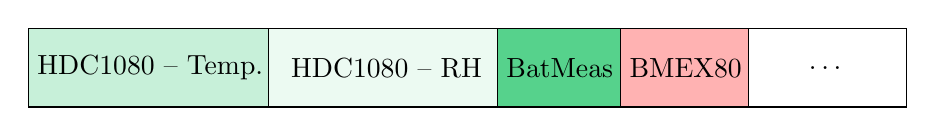
\begin{tikzpicture}
 \node[draw,fill=SeaGreen3!30!,minimum height=1cm,minimum width = 3cm,xshift=0cm](10/5){HDC1080 -- Temp.};
 \node[draw,fill=SeaGreen3!10!,minimum height=1cm,minimum width = 3cm,xshift=3cm](10/5){HDC1080 -- RH};
 \node[draw,fill=SeaGreen3!90!,minimum height=1cm,minimum width = 1cm,xshift=5.2cm](10/5){BatMeas};
 \node[draw,fill=red!30!,minimum height=1cm,minimum width = 1cm,xshift=6.8cm](10/5){BMEX80};
 \node[draw,fill=white,minimum height=1cm,minimum width = 2cm,xshift=8.6cm](10/5){\dots};
\end{tikzpicture}

The resulting frame is then transmitted using enabled communication interfaces (e.g. LoRa). 

To properly decode and interpret received data, you need to know:
\begin{itemize}
  \item list of enabled modules and their order (can be obtained from command line -- see Section \ref{sec:terminal})
  \item the module data length and format -- see the module documentation in AppNote 006: KETCube Upstream Modules \cite{ZCU:KETCubeAppNote006:09-2019}
\end{itemize}

% =================

\clearpage
\section{KETCube Terminal}\label{sec:terminal}
When programmed by the supplied software stack, the KETCube serial line called {\it KETCube Terminal} is available on USART1 (IO1 and IO2) -- see Figure \ref{fig:terminal:putty}. KETCube Terminal allows to configure KETCube modules (e.g. HDC1080, batVoltage, LoRa ...) and module parameters (e.g. devEUI, appKEY, ... for LoRa module). The KETCube terminal is case-sensitive.

The Terminal commands follow the hierarchical tree arrangement. The basic help including root commands is printed after device reset. The command {\tt help} can be used anytime to display root commands.

Inline help is displayed when {\tt [TAB]} key is pushed (e.g. write “s{\tt [TAB]}” and all commands with leading “s” will be printed -- these are: “set” and “show”). Inline help is usefull especially for commands hidden deeply in the tree structure.

To display list of modules use {\tt list} command. Commands {\tt enable}/{\tt disable} are used to turn ON/OFF KETCube modules (e.g. {\tt enable HDC1080}). When module is enabled, it starts to perform defined operation (e.g. measure RH and Temperature and send results through LoRa). 

The {\tt enable} command can be additionally used for debugging -- the second (optional) parameter of the command sets the module {\it severity level}. The {\it severity levels} are: {\it NONE (1)}, {\it ERROR (1)}, {\it INFO (2)} and {\it DEBUG (3)}. The {\it severity level} defines the amount of information provided by the specified module to the {\it terminal} interface. The default  {\it severity level} is {\it ERROR}. Use the following command to enable {\tt HDC1080}, while setting the {\it severity level} to {\it INFO}: {\tt enable HDC1080 2}.

Commands {\tt show}/{\tt set} are used to show/set KETCube settings (e.g. {\tt show LoRa devEUI}). Parameters are saved into on-chip EEPROM and take effect after the device reset (command {\tt reload} or power-cycle).

Commands {\tt showr}/{\tt setr} are used to show/set KETCube running settings (e.g. {\tt show LoRa devEUI}). Parameters are saved into RAM and take effect immediately.

The command history is available through {\tt <} and {\tt >} keys.

\marginlabel{\captionof{figure}{KETCube Terminal in Putty}\label{fig:terminal:putty}}
\raisebox{-\height}{\includegraphics[width=0.5\paperwidth]{ketCube_terminal_putty.png}}

\clearpage 

\subsection{Default KETCube Terminal Settings}

\begin{itemize}
  \item Tx PIN: PA9
  \item Rx PIN: PA10
  \item Speed: 9600 bps
  \item Data bits: 8
  \item Stop bits: 1
  \item Parity: No
  \item HW Flow control: No
  \item End-of-line: CR+LF or LF
\end{itemize}

\subsection{KETCube Remote Terminal}
When programmed by the supplied software stack, the {\it KETCube Remote Terminal} feature is available in KETCube. The {\it KETCube Remote Terminal} allows to execute KETCube commands remotely. Only the LoRaWAN network is currently supported (loraserver.io with MQTT interface was the test platform). Note, that the remote execution is enabled for ``safe'' commands only.

To control KETCube over LoRaWAN, you need a well-configured KETCube connected to the LoRaWAN network (reliable downlink is required). The {\it KETCube Remote Terminal} tool\footnote{\url{https://github.com/SmartCAMPUSZCU/KETCube-remote-terminal}} is used to configure KETCube remotely.

The {\it KETCube Remote Terminal} uses a configuration file \docFileName{config.ini}, where connection settings to the LoRaWAN application server are defined (e.g. server address, timeout, Rx and Tx topics). After writing settings into \docFileName{config.ini}, the {\it KETCube Remote Terminal} tool can be executed:

\begin{Verbatim}[frame=single, fontsize=\small]
$ ./ketcube-remote-terminal
\end{Verbatim}

The tool accepts KETCube commands in the same form as the KETCube serial Terminal. Note, that the response to the command may be delayed significantly, depending on the KETCube and the network settings and the link reliability. 

Due to increased latency given by network communication, {\it KETCube Remote Terminal} tool implements the {\it batch mode} allowing the command sequence execution:

\begin{Verbatim}[frame=single, fontsize=\small]
!batch
enable ADC
disable TxDisplay
set core basePeriod 360000
!commit
reload
\end{Verbatim}

% ============================




% ============================

\clearpage
\bibliographystyle{IEEEtran}
\bibliography{IEEEabrv,resources/sources}

% ============================

%
% Include this license into all KETCube-related documentation
%
%

\clearpage

~

\vfill

\section*{Important Notice}

\subsection*{Copyright}
\copyright ~2018 University of West Bohemia in Pilsen\\
All rights reserved.

\subsection*{Developed by}
The SmartCAMPUS Team\\
Department of Technologies and Measurement\\
Faculty of Electrical Engineering\\
www.smartcampus.cz/en $\mid$ www.zcu.cz/en

\subsection*{License\footnotemark}
\footnotetext{{\it University of Illinois/NCSA Open Source License} (\url{https://opensource.org/licenses/NCSA}) -- similar to {\it Modified BSD License}}

Permission is hereby granted, free of charge, to any person obtaining a copy of this software and associated documentation files (the “Software”), to deal with the Software without restriction, including without limitation the rights to use, copy, modify, merge, publish, distribute, sublicense, and/or sell copies of the Software, and to permit persons to whom the Software is furnished to do so, subject to the following conditions:

\begin{itemize}
    \item[--] Redistributions of source code must retain the above copyright notice, this list of conditions and the following disclaimers.
    \item[--] Redistributions in binary form must reproduce the above copyright notice, this list of conditions and the following disclaimers in the documentation and/or other materials provided with the distribution.
    \item[--] Neither the names of The SmartCAMPUS Team, Department of Technologies and Measurement and Faculty of Electrical Engineering University of West Bohemia in Pilsen, nor the names of its contributors may be used to endorse or promote products derived from this Software without specific prior written permission. 
\end{itemize}
THE SOFTWARE IS PROVIDED “AS IS”, WITHOUT WARRANTY OF ANY KIND, EXPRESS OR IMPLIED, INCLUDING BUT NOT LIMITED TO THE WARRANTIES OF MERCHANTABILITY, FITNESS FOR A PARTICULAR PURPOSE AND NONINFRINGEMENT. IN NO EVENT SHALL THE CONTRIBUTORS OR COPYRIGHT HOLDERS BE LIABLE FOR ANY CLAIM, DAMAGES OR OTHER LIABILITY, WHETHER IN AN ACTION OF CONTRACT, TORT OR OTHERWISE, ARISING FROM, OUT OF OR IN CONNECTION WITH THE SOFTWARE OR THE USE OR OTHER DEALINGS WITH THE SOFTWARE. 

\end{document}

